%%%%%%%%%%%%%%%%%%%%%%%%%%%%%%%%%%%%%%
%%  
%% Chapter 3: Running on a target device
%%
%%%%%%%%%%%%%%%%%%%%%%%%%%%%%%%%%%%%%%

\def\ArtDir{03.Target/figures}%
 
\chapter{Running on a target device}
\label{chapter:target}

As seen with the matrix multiplication example at the end of the previous chapter, there is a long directive we can add to our loops to run on the target device.
We will break this big directive down and consider the different parts of the following three chapters.
It is divided into three parts: transferring execution from the host to the device, running in parallel on the device once execution is happening there, and finally managing the movement of data between the host and device.
OpenMP has different constructs and clauses for performing each of these tasks.
When programming heterogeneous devices, particularly GPUs, it is often best to think about these different aspects separately to make things easier to grapple with.

This chapter will cover the first of these topics, along with the implicit data movement rules; with this knowledge we'll have a first program running on the device, although it won't be very fast.
Recalling the matrix multiplication example from the previous chapter shown again in Figure~\ref{code:matmulTarget}, this chapter will look what happens for the \Code{#pragma omp target} part of the directive.

\begin{CodeExample}%
{\textbf{Matrix Multiplication program} --\small This program will multiply two matrices $A$ and $B$
to produce a third $C$ which has been set to zero, running on the target device.
All arrays have been previously allocated in stack memory.
}%
{code:matmulTarget}
\begin{lstlisting}
void matmul(int Ndim, int Mdim, int Pdim,
            float A[Ndim][Pdim], float B[Pdim][Mdim], float C[Ndim][Mdim]) {

  #pragma omp target teams distribute parallel for simd collapse(2)
  for (int i = 0; i < Ndim; i++) {
    for (int j = 0; j < Mdim; j++) {
      for(int k = 0; k < Pdim; k++) {
	C[i][j] += A[i][k] * B[k][i];
      }
    }
  }
}
\end{lstlisting}
\end{CodeExample}

The remaining part of the directive is discussed in the next chapter on parallelism (Chapter~\ref{chapter:parallelism}).


\section{Host/device model}
\label{sec:host_device_model}
%% Original notes:
%% \begin{itemize}
%%   \item Host with target attached.
%%   \item Target has its own memory space.
%%   \item Can have more than one target, device() clause.
%%   \item Data moved between host and device by implicit rules and explicit directives.
%% \end{itemize}

When an OpenMP program begins running, it starts executing on the host processor.
This host processor is usually a CPU.
This initial thread is essentially the serial program that is running before any OpenMP directives are encountered.
The host processor has a memory space, which is shared between all threads running on the host processor.

Connected to this host are zero or more target devices. These target devices could be GPUs or other accelerators.
They each have their own memory space, which is distinct from the memory space of the host processor or any other device.
This means that data in our programs will be stored either in host memory or device memory.
OpenMP provides us with implicit rules for automatic data transfer along with explicit controls for the transfer of data between these memory spaces.
If the hardware supports it, OpenMP can also operate with a unified view of memory where the whole system sees a single memory space available to all; a topic we discuss in chapter~\ref{chapter:memory}.

In Figure~\ref{fig:host_device} we show a host with three connected target devices.

\begin{figure}[t]
\centerline{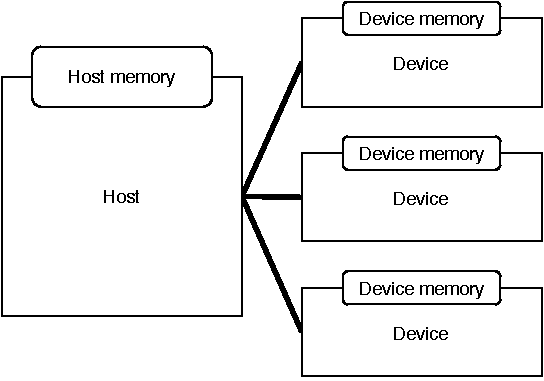
\includegraphics[width=200pt]{\ArtDir/host_device.pdf}}
\caption[The OpenMP host/device model consits of a host processor (typically a CPU) where execution begins, with zero or more attached target devices.
Data and execution can be offloaded from the host to the target device.
The memory spaces are distinct.]
{The OpenMP host/device model consists of a host processor (typically a CPU) where execution begins, with zero or more attached target devices.
Data and execution can be offloaded from the host to the target device.
The memory spaces are distinct.}
\label{fig:host_device}
\end{figure}


We can query the OpenMP runtime for the number of available target devices in the system using the \Code{omp\_get\_num\_devices()} API call.

\begin{verbatim}
#include <stdio.h>
#include <omp.h>

int main() {
  printf("There are %d devices\n",
    omp_get_num_devices());
}
\end{verbatim}

The devices themselves are numbered between zero and the number returned by this API call.
The final device with value equal to the value returned by \Code{omp\_get\_num\_devices()} is the \emph{initial device}.
The initial device is the host itself.
This means we can use the same mechanisms for programming attached target devices as we can for programming the host by treating it as a device.

One of the devices will be chosen by the implementation to be the \emph{default device}.
This is the device that will be used unless another is explicitly chosen.
The device used can be chosen using clauses or calls to APIs.
In general we will not choose a device and so the majority of code we show throughout this book will run on the default device.

In Section~\ref{sec:multi_gpu} we will explore how to use OpenMP to program systems with multiple devices, where devices will be chosen using this simple numbering scheme above.

This model of a host with some attached devices, each with their own separated memory space, is a model commonly found in heterogeneous programming models.

\subsection{Target construct offloading execution}

% Original notes
%% \begin{itemize}
%%   \item Target directive.
%%   \item Defines movement of execution to the target device.
%%   \item Host waits for the region to finish.
%%   \item Devices are numbered from 0 to this number, so can loop over them, using the device clause.
%%   \item Don't want too much detail on the tasking model here because will go into it in Chapter~\ref{chapter:async}. It's not relevant for getting starting this early on.
%% \end{itemize}

OpenMP uses the \Code{target} construct for offloading execution to a device.
The majority of the constructs we use in this book are based on this \Code{target} construct.
The code in the structured block associated with the \Code{target} construct is executed by the target device instead of the host.
This code that resides in this block is known as the \emph{target region}.

\begin{verbatim}
#pragma omp target
{
  // Code to run on the device
  // This code is the target region.
}
\end{verbatim}

When the host encounters this \Code{target} construct, execution is transferred to the device which completes the work in the target region.
By default, the host waits until the region has completed, at which point execution is returned back to the host.
This is shown in Figure~\ref{fig:target_region}.

\begin{figure}[t]
\centerline{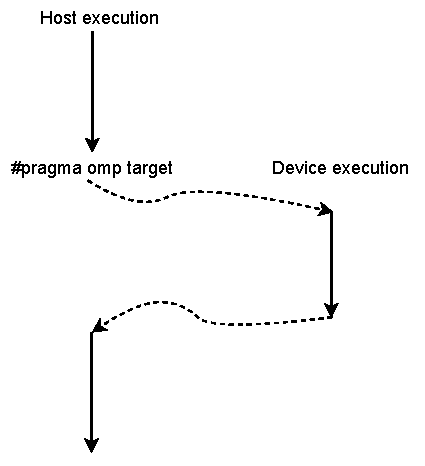
\includegraphics[width=200pt]{\ArtDir/target_region.pdf}}
\caption{Illustration of transfer of execution from the host to the device at a \Code{target} construct.}
\label{fig:target_region}
\end{figure}

OpenMP uses a task mechanism to carefully define the transfer of control.
We will defer the details of this until Section~\ref{sec:async} where they will be covered in the context of allowing the host to do useful work whilst waiting for the target region to complete.
For now however, we can be contented with the fact that execution is transferred to the device, and continues again back on the host when the work on the target device is done.

Consider the vector addition example from the previous chapters.
How can we run this on the target device?
With the addition of a single \Code{target} construct we can run the loop on the device instead of the host.
In Figure~\ref{code:vaddTarget} we add the construct to line 8.
This is a big step --- we are now using the accelerator to run our code.
The target region consists of all the code from lines 9--11: the \Code{for} loop.
The host CPU will wait until the loop finishes executing on the device.

\begin{CodeExample}%
{\textbf{Vector Add program} --\small This program will add two vectors of length $N$
to produce a third vector, running on the target device.
}%
{code:vaddTarget}
\begin{lstlisting}
#define N 4000;

int main()
{

   float A[N], B[N], C[N];

   #pragma omp target
   for (int i = 0; i < N; i++) {
      C[i] = A[i] + B[i];
   }
}	  
\end{lstlisting}
\end{CodeExample}

When execution of the target region begins on the device, the execution only occurs in a single thread.
This means the target device will execute the target region in serial.
Chapter~\ref{chapter:parallelism} will show the constructs needed to run in parallel on the device.

For the matrix multiplication example shown at the start of this chapter (Figure~\ref{code:matmulTarget}), execution is transferred in the same way.
The host enters the function, and encounters the \Code{target} construct.
Execution is then transferred to the device for the target region scope: the end of the closely nested \Code{for}-loops.
Once execution has finished, it reverts back to the host to continue execution, and return from the function in the example.


There is another outstanding question.
How does the data move onto the device?
We know they are separate memory spaces, so the host data doesn't yet exist on the device.
When the \Code{target} construct is encountered on the host, in addition to transfer of execution, there may be the transfer of \emph{data} between the host and device.
The device and host do not share a memory space, so data must be copied between them.
These data transfers can happen at just a few specific places, the first of which is the beginning and end of a target region.
We will cover some of the memory movement now with the goal of showing our first OpenMP programming correctly running on the device.
While Chapter~\ref{chapter:parallelism} will cover the parallelism on the device, Chapter~\ref{chapter:memory} will expand on the data transfer rules to include allocatable data (on the heap or free store).

For the vector add example in Figure~\ref{code:vaddTarget}, data transfer will also happen on line 8.
The target construct moves data and execution from the host to the device.
In this example, we'll show that all the data we need will be transferred by the implicit rules built into OpenMP.
The example will correctly run on the target device, but we probably expect the performance to be slow: we have to account for data movement and the serial execution on a target device which was likely designed for throughput.
Over the next few chapters, we'll improve the performance significantly by exposing the parallelism of the loop and managing the data transfer.
Next we will explain how the data moves in the vector add example.


\section{The target memory environment and implicit mapping rules.}
% Original notes
%% \begin{itemize}
%%   \item target directive also triggers data movement as well as execution.
%%   \item first place where data movement is allowed, and will introduce the others at appropriate points.
%%   \item Different kinds of data we want to move: scalars, (stack) arrays, heap data/pointers, structures.
%% \end{itemize}

The target device has its own memory space, distinct from the host.
The target memory space is called the \emph{device data environment}.
In order for the target region executing on the device to do anything useful, we must copy data from the host to the device data environment, execute using it, and the copy it back to the host.
The \Code{target} directive is one such place where this data transfer might occur; there are a few other places that we will introduce later that help to minimizing the transfers.

OpenMP uses a combination of implicit rules and explicit clauses and constructs to copy data between the host memory space and the device data environment.
We will first introduce the implicit rules, where data is automatically moved between the host and device.

At the start of a target region, data may be copied from the host \emph{to} the device.
At the end of a target region, data may be copied back \emph{from} the device to the host.
The direction of the memory transfers in OpenMP are always from the perspective of the host.
Data is either copied to the device, or from the device.

Recall that the target region is described by the \Code{target} construct.
The following code snippet shows where the transfers occur for the \Code{target} construct.
The structured block between the curly braces is the target region offloaded to the device for execution.
\begin{verbatim}
#pragma omp target
{ // <-- copy data to the device

} // <-- copy data from the device
\end{verbatim}

The implicit rules for what variables are copied at this stage are limited to scalars, stack arrays and structures (\Code{struct}) with complete types.
We will explain the most commonly occurring types of variables and what happens automatically at the beginning and end of a target region.
The copying of data to and from the target device is known as \emph{mapping}.
We might also say a variable is \emph{mapped}.
There are a number of ways a variable can be mapped, and we will go through some common examples here.
The full details can be found in \S2.21.7 of the OpenMP 5.1 specification.

Data allocated on heap or free store must be explicitly copied, and we will show how to do this later in Chapter~\ref{chapter:memory}.
The main thing to remember is that any data referred to with a pointer \emph{will not} to transferred automatically.

\subsection{Scalar variables}

% Original notes
%% \begin{itemize}
%%   \item Mapped as firstprivate.
%%   \item Example: {\tt int N; double x;}
%%   \item a scalar struct, as long as it is a complete type
%%   \item {\bf Not} copied back to the host at end of target region.
%% \end{itemize}

Programs perform some operations on data, and that data can take various forms.
Usually programs contain lots of scalar variables.
These variables hold a single piece of data, and they are given a name.

For OpenMP programs, scalar variables are just as they are in the base language of the program, be it C, C++ or Fortran.
For a C program therefore, scalar variables will have one of the basic data types from the C language: \Code{char}, \Code{int}, \Code{float}, \Code{double}, etc.
(A scalar variable can also be a pointer --- \Code{int *} --- however we will discuss these later.)

OpenMP implicitly makes scalar variables available inside the target region, so that they are automatically copied to the device when the target construct is encountered.
For example, consider the program in Figure~\ref{code:scaleTarget}.
This code multiplies the array \Code{A} by a scalar floating point number \Code{alpha}.
We will deal with how \Code{A} appears on the device in a moment.
For now, we consider just the scalar variable \Code{alpha}.

\begin{CodeExample}%
{\textbf{Scaling program} --\small This program will multiply a vector of length $N$
by a constant in place, running on the target device.
}%
{code:scaleTarget}
\begin{lstlisting}
#define N 4000;

int main()
{

   float A[N];
   float alpha = 2.0;

   #pragma omp target
   for (int i = 0; i < N; i++) {
      A[i] = A[i] * alpha;
   }
}	  
\end{lstlisting}
\end{CodeExample}

The data held in scalar variables is copied to the device on entry to the target region.
OpenMP transfers them as \Code{firstprivate} (recall Section~\ref{sssec:data_sharing}).
This means that all parallel threads which will run on the target device have their own copy of the variable.
It also means that the variable is initialized with the original value (\Code{firstprivate} rather than \Code{private} is used so the value of the variable is retained).
This is important: we know our \Code{alpha} variable will contain the number \Code{2.0} as this is what the variable was set to on the host before it encountered the target construct.

With scalar variables being mapped from the host to the target device as \Code{firstprivate} we much also consider what happens to those variables at the end of the target region.
As with all \Code{private} (and by extension \Code{firstprivate}) variables, the value of the original variable (the one on the host) will become undefined outside of the associated construct.
Here this means that once the target region is executed on the device and control is returned back to the host, the value of \Code{alpha} should be considered undefined.

We can extend this further with the small snippet of code in Figure~\ref{code:firstprivateTarget}.
The \Code{alpha} variable will be copied to the device at the start of the target region on line 7 of the program.
On line 9, the copy of the variable on the device is updated to a new value (\Code{1.0}), but this update will not necessarily be seen on the host device.
We have no way of knowing what the value shown by the \Code{printf} on line 12 will be.
By mapping scalar variables as \Code{firstprivate} any updates to those variables will not be seen by the host.

\begin{CodeExample}%
{\textbf{Forgotten value program} --\small This program sets a \Code{firstprivate} variable
inside a target region.
}%
{code:scaleTarget}
\begin{lstlisting}
#include <stdio.h>

int main()
{
   float alpha = 2.0;

   #pragma omp target
   {
      alpha = 1.0;
   }

   printf("alpha=%f\n", alpha);
}	  
\end{lstlisting}
\end{CodeExample}

For those of you who may be familiar with the kernel-style programming language of OpenCL, passing scalar variables as private variables is equivalent to passing them directly as arguments to the kernels.
For some context, imagine the target region was outlined into a new function; what arguments would that function take?
For scalar variables we can think as if they are passed by value to this outlined function.


Lets look back at the matrix multiplication program from Figure~\ref{code:matmulTarget}.
Of all the variables in this snippet of code, there are three scalar variables declared before the target construct: \Code{Ndim}, \Code{Mdim} and \Code{Pdim}, the sizes of the matrices.
These variables will be mapped \Code{firstprivate}, and a copy of the data held in the variables will be transferred to the device.
These variables are not changed inside the target region, but if they were to be their new values would be lost at the end of the target region.

The loop iteration variables are declared \emph{inside} the target region and so follow the usual scoping rules for all OpenMP programs.
They need no special treatment.
The other variables defined before the target construct in our matrix multiplication program are not scalar variables --- the are the matrices stored on the stack as arrays.
We will come to what happens to them in the next section.

In summary, scalar variables will be copied automatically to the target device at the start of the target region.
Scalar variables are those which have a basic type in the base language.
They will be initialized on the device with the value they held on the host prior to encountering the target construct.
Any updates to the variable will not be made available to the host because it is private.

This behaviour also means that we need a different mechanism to return scalar values from the device back to the host.
We will show how this is done in Chapter~\ref{chapter:memory}.


\subsection{Stack arrays and derived types}

%% Original notes
%% \begin{itemize}
%%   \item Fixed sized stack arrays.
%%   \item Example: {\tt double arr[1024];}
%%   \item Complete types. Arrays of structs if complete type.
%%   \item Copied to device at start of target region, copied back at the end.
%%   \item Define mapping.
%%   \item Host not allowed to use copy in the meantime (with further details on this in Chapter~\ref{chapter:async}\dots).
%%   \item Data shared between {\bf all threads} on a device.
%% \end{itemize}

An \emph{incomplete type} in C is a variable whose size is not known at compile time.
Examples are structures (and unions) where the members are not yet specified and array types with unknown dimension.
For example, the integer array type \Code{int[]} is an incomplete type.
To make it \emph{complete}, the size of the array needs to be specified, i.e.\ \Code{int[1024]}.
Now the compiler knows how much memory to allocate for variables of that type.

We may commonly run into arrays of numbers in codes that we want to run on the device.
For now, we assume they are allocated on the stack, being declared in the code using an array type with a known extent.
Later we will deal with arrays of unknown size which are allocated on the heap and accessed via pointers.

Arrays allocated on the stack are variables, but they are not scalar variables as they contain other variables.
We can use \Code{struct} to define a composite data type made up of other data types.
Although these are not scalar types, OpenMP will transfer the data held in these variables automatically.
The behaviour is different to scalars which are mapped \Code{firstprivate}.

Non-scalar variables with complete types will be copied to the device at the start of the target region, \emph{and} copied back to the host at the end of the target region.
We can update the device copy of that data inside the target region, and the updated values will then be retained.
The data will also be \emph{shared} between any parallel threads that might be running inside the target region.
This is quite different to the behavior for scalar variables, where the data was copied and privatized, and not copied back at the end of the region.

The vector addition example we showed in Figure~\ref{code:vaddTarget} utilizes this implicit behaviour.
The arrays \Code{A}, \Code{B} and \Code{C} are of type \Code{float[4000]}.
The \Code{N} is defined in the preprocessor, so all references to it are replaced with the value \Code{4000}.
This means those arrays will be copied to the device at the start of the target region.
The code inside the target region updates the array \Code{C}, and this array will be copied back to the host at the end of the device execution.
We will also copy back \Code{A} and \Code{B} too as they follow these same rules of being copied at the start and end, even though we did not update them.

This is our first example of what OpenMP calls \emph{mapping}.
Variables are mapped from the host memory space in and out of the device memory space.
The variables should be considered simultaneously the same and separate!
They share the same name, and can only be accessed in their respective places.
OpenMP is allowed to use the same storage if possible, but it might not.
When the variable is used on the device, then it is not correct to use it on the host at the same time, and vice versa.

Variables are mapped to the device at the start of the target region and mapped from the device at the end of the target region.
When the variables are like our stack arrays (i.e.\ variables with complete type), OpenMP implicitly copies the data between the host and device when they are needed.
This means OpenMP will allocate memory on the device, copy the data from the host into that new allocation at the start of the target region.
The process is reversed at the end of the target region: the data is copied back to the host variables and then deallocated.
The allocation/deallocation follows reference counting semantics.

Structures containing multiple types are also copied to and from the device at the start and end of the target region respectively.
The variable along with the component parts are all mapped the same way.
Including just the structure variable on the target construct will automatically map the structure members too.


\begin{CodeExample}%
{\textbf{Structure mapping program} --\small This program shows the mapping of a C \Code{struct} variable.
}%
{code:structMapping}
\begin{lstlisting}
#include <math.h>

struct complex {
  float real;
  float imag;
};

int main()
{
   struct complex data = {.real = 1.0f, .imag = 2.0f};
   float len[1];

   #pragma omp target
   {
     len[0] = sqrtf(data.real * data.real + data.imag * data.imag);
   }

}	  
\end{lstlisting}
\end{CodeExample}


Figure~\ref{code:structMapping} shows a structure to hold two single-precision floating point numbers, which we use to represent a complex number.
As a slightly contrived example, we wish to use the target device to complete the absolute value of the complex number and store the result in an array stored on the stack.

We use an array here so that the value is automatically copied back, just as it is for the vector addition program.
If we used a scalar variable instead, it would be implicitly mapped \Code{firstprivate} and the value we set it to inside the target region would be lost.
By using an array (of length one), OpenMP will copy the new value back to the host automatically at the end of the target region.

The \Code{struct complex} is made up of other variables (two \Code{float}s), and is a complete type because it is made up of types of a known size.
As such, the \Code{data} variable will be copied to the device when the target construct is encountered on line 13 and copied back at the end of the target region on line 16.

If the structure contained a pointer then the structure will still be mapped in the same way as described.
However the target of the pointer will not be nor will the pointer be translated into the device memory equivalent.

We look back again at our matrix multiplication in Figure~\ref{code:matmulTarget}.
The arrays \Code{A}, \Code{B} and \Code{C} have been allocated on the stack in the calling host program.
The \Code{matmul} function definition includes the sizes of the arrays.
These arrays will be mapped to the device when the \Code{target} region is encountered.
When execution finishes on the device, they will be mapped from the device back to the host again.
The \Code{C} array on the host will contain the result of the matrix multiplication, which was performed on the device.


\subsection{Pointers and arrays on the heap}
%Warning: heap arrays and pointers - reference later chapter}
%\begin{itemize}
%  \item We don't introduce the map clause yet.
%  \item This is done in Chapter~\ref{chapter:memory}.
%  \item This section says that we must do something explicit for everything not covered by the implicit rules.
%  \item Examples of those would be heap arrays, and data-structures with pointers.
%\end{itemize}

What happens if our matrix multiplication function didn't use stack allocated arrays?
We might have written the function definition using pointers, for arrays allocated on the heap (using \Code{malloc()}):
\begin{verbatim}
void matmul(int Ndim, int Mdim, int Pdim, float *A, float *B, float *C);
\end{verbatim}

OpenMP doesn't know how much data is at the end of these pointers.
With the target directive as shown in Figure~\ref{code:matmulTarget}, the data in the arrays will not be copied to and from the device in this case.
We had better hope the data was already there!
We will look at how to make sure that the data is copied in Chapter~\ref{chapter:memory}.

The variables \Code{A}, \Code{B}, and \Code{C} are pointers, and there are some implicit rules in OpenMP for them.
They are mapped as zero-length arrays.

In plain terms, the pointer itself is translated, but the target of the pointer doesn't move.
This means we can use the pointer inside the target region, but dereferencing it is might be a bad idea.


\section{Example: Walking through vector addition}
% Original notes
%% \begin{itemize}
%%   \item Takes vector add example from Chapter~\ref{chapter:overview}.
%%   \item Arrays are allocated on the stack, so follows implicit mapping rules.
%%   \item Example will simply transfer execution.
%%   \item Parallelism comes in Chapter~\ref{chapter:parallelism}.
%%   \item In OpenCL, have to deal with the host API copying buffers to/from host and device before we can run a meaningful kernel. Thinking in OpenCL might help here.
%% \end{itemize}

You have seen the vector addition code a number of times in this chapter.
In this section we'll walk through the execution of the vector addition program, line by line.
This example puts together everything in this chapter and sets the scene for later chapters where we are able to exploit the parallelism of the target device itself.

The program is listed in Figure~\ref{code:vaddTargetWalkthrough}.
We will refer to the line numbers in this figure.
The overall goal of the program is to add the elements of two arrays together and storing the results in a third array.
The input arrays here are initialized to \Code{1.0} and \Code{2.0} for every array entry.
The program sets the elements of the output array to their sum: $1+2=3$.

Line 2 sets the size of the arrays.
This is done by the C pre-processor just before compile time.
Every reference to \Code{N} in the program is replaced by the value \Code{4000}.
We do this so that we're able to allocate our three arrays on line 8.
The arrays are of a known, fixed, size.
The C compiler will allocate the memory on the stack.
For an OpenMP program running on target devices this means we're able to use the implict data transfer rules and we do not need to explicitly manange the different memory spaces.
OpenMP takes care of stack arrays for us.

The host initalizes the arrays to their starting values on lines 10--12.

So far we've just written a standard serial C program.
But on line 16 we have our first (and only) OpenMP construct: the \Code{target} directive.
This construct is associated with a the structred block of code underneath it, which forms the target region.
The target region in our vector addition program is the \Code{for} loop on lines 17--19.
The target region will be executed on the target device.
The target region will run in serial on the target device because we have not exposed any parallelism through the various constructs available in OpenMP for expressing the concurrency.
The for-loop then is run in sequential order on the device.

The target construct also invokes some transfer of data at the beginning and the end.
Variables used in the target region need to be made available on the device in the device data environment.
There are only four variables in this example: three arrays \Code{A}, \Code{B} and \Code{C}, and one scalar integer \Code{i}.
Note that \Code{N} is replaced by a numerical literal during compilation, so is not a variable.

The variable \Code{i} is declared inside the target region.
It will of course be available for use on the target device.
There is no additional parallelism to worry about at this stage, so there is only one copy of this variable, and it exists on the device only.
The host has no access to or copy of this variable \Code{i}.

The three arrays exist on the host, and are found in the stack.
They are of a known extent, and so form a complete type.
OpenMP will therefore implicitly map these arrays to the device for us.
This will happen on line 16 as part of the target construct.
Space will be allocated in the device data ennvoronment (in the device memory space) and the values of these arrays as found on the host will be copied over to these new device arrays.
This means both the host and device have identical copies of the three arrays just before execution is transferred.

Once this data is transferred, execution is transferred.
The device runs lines 17--19.

After the execution of the for-loop has finished, the target region ends, and execution must be returned to the waiting host.
Just before this happens, the target construct might copy back any variables that were implicitly mapped.
In this program, this is the three arrays.
These data held in these arrays is copied back to the arrays on the host.
The host copy of array \Code{C} is set to whatever value is in the device code of array \Code{C}: the number \Code{3.0}.
The other two arrays will also be copied back to the host.

Once this data transfer has finished, the host continues execution on line 20, which simply ends the program.


\begin{CodeExample}%
{\textbf{Vector Add program} --\small This program will add two vectors of length $N$
to produce a third vector, running on the target device.
}%
{code:vaddTargetWalkthrough}
\begin{lstlisting}
// Array length, defined at compile time
#define N 4000;

int main()
{

   // Allocate arrays on the stack
   float A[N], B[N], C[N];

   for (int i = 0; i < N; i++) {
     A[i] = 1.0; B[i] = 2.0; C[i] = 0.0;
   }

   // Transfer execution to the device
   // Also map arrays to and from the device
   #pragma omp target
   for (int i = 0; i < N; i++) {
      C[i] = A[i] + B[i];
   }
}	  
\end{lstlisting}
\end{CodeExample}

\section{Advanced: Corresponding Variables}
Into specification details, explain how the term corresponding variable.
Reference counting.


%-----------------------------------------------------------------------
%------------------------- From Next Step ------------------------------
%-----------------------------------------------------------------------
\section{From The Next Step Chapter 6}
\subsection{Devices and Accelerators}
\label{sec:06.devices}
\index{Accelerators}

Typically, the motivation for running code on a heterogeneous architecture is
to execute parts of a program on an \emph{accelerator}.  As the name implies,
the desire is to dramatically improve the performance of a program by
leveraging the specialized hardware capabilities of accelerator devices.  

\index{Accelerators!Processing element}
\index{Accelerators!Device}
\index{Accelerators!Host device}
\OMP\ provides the means to distribute the execution of a program across
different devices in a heterogeneous architecture.  A device is a computational
resource where a region of code can execute.  Examples of devices are GPUs,
CPUs, DSPs, FPGAs or other specialized processors.  \OMP\ makes no distinction
about the specific capabilities or limitations of a device.  Devices have their
own threads which cannot migrate across devices.  Program execution begins on
the \emph{host device}.  The host device offloads the execution of code and
data to accelerator devices.\footnote{\OMP\ uses the term \emph{target}
devices.}  Devices have access to memory where variables are stored.  The
memory may or may not be shared with other devices.

\index{OpenMP constructs!Target}
\index{Accelerators!Target}
As shown in the code fragment in Figure~\ref{figure:chapter6-device-v1}, the
\code{#pragma omp target} directive defines the target region spanning lines
$1-6$.   When a host thread encounters the \code{target} construct on line
$1$, the target region is executed by a new thread running on an accelerator. 

\begin{figure*}[!b]
\begin{verbatim}
1 #pragma omp target map(a,b,c,d)
2 {
3   for (i=0; i<N; i++) {
4     a[i] =  b[i] * c + d;
5   }
6 } // End of target
\end{verbatim}
\caption{ \textbf {Code fragment with one target region} -- \small
          The target region is executed by a thread running on
          an accelerator.
         }
\label{figure:chapter6-device-v1}
\end{figure*}

By default, the thread that encounters the \code{target} construct waits for
the execution of the target region to complete before it can continue executing
the code after the \code{target} construct.

\index{Mapped variable}
Before the new thread starts executing the target region, the 
variables \code{a}, \code{b}, \code{c}, and \code{d} are \emph{mapped} to the accelerator.
Mapped is the concept that \OMP\ uses to
describe how variables are shared across devices.

%Before the new thread starts executing the target region, the original
%variables $a$, $b$, $c$, and $d$ are \emph{mapped} to corresponding variables.
%Storage for the corresponding variables is allocated in the accelerator's
%memory and initialized with the value of the original variables.  When the
%execution of the target region is completed, the value of the corresponding
%variables $a$, $b$, $c$, and $d$ are assigned to the original variables in the
%host device's memory and the storage for the corresponding variables is
%released.

Very often the code that we wish to accelerate already includes \OMP\ pragmas.
We can place a \code{target} directive before a structured block that contains
\OMP\ constructs.  In the code fragment shown in
Figure~\ref{figure:chapter6-device-v2}, the target region is executed by a new
thread on an accelerator.  However, the new thread immediately encounters a
\code{parallel for} construct and a team of threads is created that work
together to execute the iterations of the subsequent loop.

\begin{figure*}[!tbhp]
\begin{verbatim}
1 omp target map(a,b,c,d)
2 {
3   #pragma parallel for
4   for (i=0; i<N; i++) {
5     a[i] =  b[i] * c + d;
6   }
7 } // End of target
\end{verbatim}
\caption{ \textbf {Augmented code fragment with a parallel region} -- \small
          The parallel region is executed by a team of threads running
          on an accelerator.
        }
\label{figure:chapter6-device-v2}
\end{figure*}

The heterogeneous features of \OMP\ fall into two general categories: program
execution and data management.  In the following sections, we will cover each of
these categories in more detail.

%-----------------------------------------------------------------------
%------------------------- New subsection ------------------------------
%-----------------------------------------------------------------------
\subsection{Heterogeneous Program Execution}
\label{sec:06.execution-model}
% Ruud - Changed to "m" for consistency.
\index{Accelerators!Execution model}

\index{Accelerators!Device constructs}
This section describes the \OMP\ heterogeneous program execution model.
The device constructs, clauses, and new environment variable
listed below are used to determine where (on which device) and how regions of a
program are executed on a heterogeneous architecture: 

\begin{itemize}
  \item Target Construct
  \item Target Teams Construct
  \item Declare Target Construct
  \item Distribute Construct
  \item Device and Nowait Clauses
%  \item Runtime Functions
%  \begin{itemize}
%    \item \code{omp_get_default_device}
%    \item \code{omp_set_default_device}
%    \item \code{omp_is_initial_device}
%    \item \code{omp_get_num_devices}
%    \item \code{omp_get_num_teams}
%    \item \code{omp_get_team_num}
%  \end{itemize}
  \item \code{OMP_DEFAULT_DEVICE} Environment Variable
\end{itemize}

Of these, the \code{target} and \code{target teams} constructs are the
most important as they are used to select which parts of a program are run on
an accelerator.  When a function name appears in a \code{declare target}
construct, it indicates that the function is expected to be called from code
executing on an accelerator, thus causing the compiler to generate a
device-specific version of the function.  

The heterogeneous execution model concepts are covered in this section.  The
complete syntax and semantics of the \code{target}, \code{target teams}, and
\code{declare target} constructs are covered in detail in Sections
\ref{sec:06.target-construct}, \ref{sec:06.teams-construct}, and
\ref{sec:06.declare-target-construct}, respectively.

On a heterogeneous architecture with
multiple accelerators, the \code{device} clause, \code{OMP_DEFAULT_DEVICE}
environment variable, and runtime functions listed in 
Section~\ref{ssec:02.new_runtime_functions_3} starting on
page~\pageref{ssec:02.new_runtime_functions_3}  
are used to choose among and query about the different devices.  
Selecting a device using these clauses and functions is described in 
Section~\ref{sec:06.which-device}.

By default, the thread that encounters a device construct waits for the
construct to complete.  However, when a \code{nowait} clause is added to a
device construct, the encountering thread does not wait, but instead continues
executing the code after the construct.  Task scheduling constructs are
used to synchronize with the completion of the device construct's execution.
The relationship between the device constructs and tasking is discussed in
this section. The \code{nowait} clause is covered in Section~\ref{sec:06.async-exec}.

%Work-sharing is how parallel computation (work) is scheduled and coordinated
%(shared) across the threads in a team of that threads that arise from a
%\code{parallel} construct.  

\index{OpenMP constructs!Target teams}
\index{Accelerators!Target teams}
The \code{target}~\code{teams} construct starts multiple thread teams running
in parallel on an accelerator.  The \code{distribute} construct is a
worksharing construct that schedules the iterations of a loop across the teams
that are started by a \code{target}~\code{teams} construct.

Combined with the \code{parallel for} and \code{simd} constructs, the
\code{distribute} construct expresses a three-level hierarchy of parallelism
across which loop iterations are spread.  Loop iterations are first distributed
to teams of threads, then to the threads in each team and, then to the SIMD
vector lanes within each thread.  This pattern of nested parallelism is
executed efficiently by many types of accelerators.

The syntax and details of the \code{distribute} construct, and its combination
with other constructs are covered in Sections \ref{ssec:06.distribute-construct}
and \ref{ssec:06.composite-worksharing-loop-construct}.

%-----------------------------------------------------------------------
%------------------------- New subsection ------------------------------
%-----------------------------------------------------------------------
\subsubsection{A New Initial Thread}
\label{ssec:06.initial-thread}
\index{Accelerators!Initial thread}

\index{Accelerators!Host device}
Recall that the thread that starts the execution of a program and executes all
of the sequential code outside of any parallel regions is the \emph{initial
thread} (see Section~\ref{ssec:01.execution_model}).  The \OMP\ heterogeneous
execution model is host-centric.  The initial thread that starts the execution
of a program is running on the host device.  In other words, the program starts
running on the host device.  Prior to \OMPfourzero\, there was only one initial thread.

\begin{figure*}[!tb]
\centering
\pdfimageresolution 400
\fbox{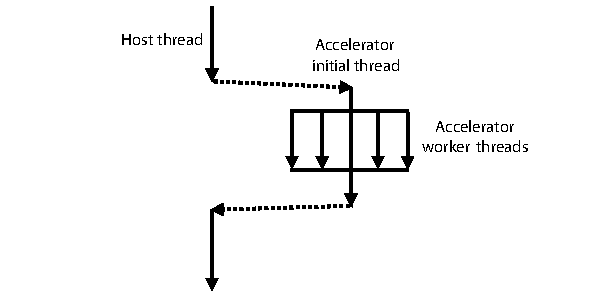
\includegraphics[clip=true,scale=1.00]
         {\ArtDir/device-exec-model.pdf}
     }
\caption{ \textbf{The heterogeneous programming model supported by OpenMP} -- \small
        Program execution begins on the host device.  When a host device
        thread encounters a \texttt{target} construct, a new initial thread 
        executes the target region.  When the initial thread encounters
        a \texttt{parallel} construct it becomes the master of a
        teams of threads.
        }
\label{figure:chapter-6-device-exec-model}
\end{figure*}

After \OMPfourzero\ and the addition of the \code{target} construct, multiple
initial threads could arise during the execution of a program.  A
\emph{target}~\emph{region} is all of the code that is dynamically encountered
during the execution of a \code{target} construct.  As shown in
Figure~\ref{figure:chapter-6-device-exec-model}, the thread that encounters a
\code{target} construct does not itself execute the target region.  Instead, a
new initial thread begins the execution of the target region.  Each
target region acts as an \OMP\ sub-program where an initial thread begins the
execution of the sub-program.  The initial thread may encounter
other parallel constructs and spawn teams of threads. 

The initial thread that executes a target region is potentially running on an
accelerator.  We say potentially because it's possible that the OpenMP
program is running on a system that has no accelerators, in which case, the
target region is executed by an initial thread running on the host device.
Even on systems where accelerators are available, if the \code{target}
construct has an \code{if} clause whose conditional expression evaluates to
\emph{false} then the initial thread executes on the host device (see
Section~\ref{ssec:06.if-clause}).  If there are multiple accelerators
available, the \code{device} clause %(see Section~\ref{ssec:06.device-clause})
can be used to select one of them.  When a \code{device} clause is not present,
the initial thread executes on the default device specified by the
\emph{default-device-var} ICV.
% Ruud - Changed to a "D" for consistency.
\index{Accelerators!Default-device-var ICV}
\index{ICV!default-device-var}

By default, the thread that encounters the \code{target} construct waits for
the execution of the target region to complete and then continues executing the
code after the \code{target} construct.  Note how this is different from a
\code{parallel} construct where the thread that encounters the construct
becomes the master thread in a team of threads that is created to execute the
parallel region.  

%-----------------------------------------------------------------------
%------------------------- New subsection ------------------------------
%-----------------------------------------------------------------------
\subsubsection{Contention Groups}
\label{ssec:06.contention-groups}
\index{Accelerators!Contention group}
\index{Accelerators!Initial thread}
\index{Contention group}

A \emph{contention group} is the set of all threads that are descendants of an
initial thread.  An initial thread is never a descendant of another initial
thread.  Each dynamically encountered \code{target} construct starts a new
contention group.  

Threads in different contention groups cannot synchronize with
each other.  This means that threads that arise from different target regions
cannot synchronize with each other.  Further, the threads in the contention
group formed by the initial thread that started the execution of the program
cannot synchronize with any threads that arise from target regions.  This
restriction effectively limits how threads in contention groups (often threads
on different devices) can interact with each other.

When threads from different contention groups execute in parallel, only
variables\footnote{The size of these variables must be less than or equal 64 bits.} 
written to atomically 
(using an \code{atomic} construct)
by a thread in one contention group can be read by a thread in another contention group, and only
if both contention groups are executing on the same device.

%-----------------------------------------------------------------------
%------------------------- New subsection ------------------------------
%-----------------------------------------------------------------------
\subsubsection{A League of Teams}
\label{ssec:06.league-of-teams}
\index{Accelerators!League}
\index{Accelerators!Contention group}
\index{Accelerators!Initial thread}
\index{Contention group}

The \code{target}~\code{teams} construct %(see Section~\ref{sec:06.teams-construct}) 
starts a \emph{league} of teams executing
on an accelerator. Each of these teams is a single initial thread executing
in parallel the subsequent code statement.  This is similar to a
\code{parallel} construct but different in that each thread is its own team: a
team of one.  Threads in different teams are in different contention groups
and, therefore, restricted in how they can synchronize with each other.  

When a \code{parallel} construct is encountered by a league, each initial
thread in the league becomes the master of a new team of threads. The result is
a league of teams where each team has one or more threads. Each team is a
contention group.  Each team of threads then concurrently executes the parallel
region.

Leagues are used to express a type of loosely connected parallelism where teams
of threads execute in parallel but with very limited interaction across teams.
We will explore this more later in Section~\ref{ssec:06.distribute-construct}
when we discuss how leagues are used in accelerated worksharing.

%-----------------------------------------------------------------------
%------------------------- New subsection ------------------------------
%-----------------------------------------------------------------------
\subsubsection{The Target Task}
\label{ssec:06.target-task}
\index{Tasking!Creation}
\index{Creation of tasks}
\index{Accelerators!Target task}

Sometimes we don't want the host thread that encounters a target region to wait
for the target region to complete.  We want the target region to execute
asynchronously so that the host thread can go off and do other work.
\OMP\ already has tasks that provide capabilities for launching and
coordinating the asynchronous execution of code regions.  Leveraging these
features, the device constructs are formulated as \OMP\ task generating
constructs. 
\index{Accelerators!Device constructs}

We have been talking in terms of threads up to this point, but recall that
threads are the entities that do work; the actual work is a task.  There is
always a task (implicit or explicit) that a thread is executing.  Tasks are
executed only by threads running on the device where the tasks were generated.

The \code{target} construct is a task-generating construct.  When a thread
encounters a \code{target} construct, it generates an explicit task that
manages the execution of the target region.  The \OMPfourfive\ specification
refers to this task as the \emph{target task}.  This is an unfortunate name as
it seems to imply that the target task is running on an accelerator, but it
is an explicit task generated on the host.  The target task is complete when
the enclosed target region is complete.

\index{Accelerators!Initial thread}
When the target task executes, the target region executes in the context of an
implicit task, called an \emph{initial task}, on the accelerator.  The initial
task is executed by the initial thread.  Before \OMPfourzero\, there was only one
initial task; the implicit task that enclosed the whole program.  However, now each
time a target region executes, a new initial task is generated on the target
device.  The target task is complete when the initial task, and thus the target
region, is complete.

\index{Accelerators!Generating task}
The task that the host thread is executing when it encounters the \code{target}
construct is called the \emph{generating task}.  It generates the target task.
Because the \code{target} construct results in a task, we now have available
all of the asynchronous execution features from \OMP\ tasking.

\begin{figure*}[!tb]
\centering
\pdfimageresolution 400
\fbox{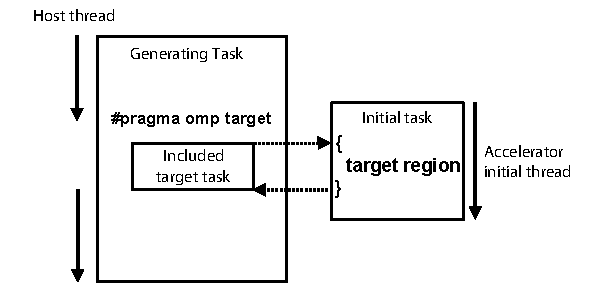
\includegraphics[clip=true,scale=1.00]
         {\ArtDir/device-task-model1.pdf}
     }
\caption{ \textbf{The target task as an included task} -- \small
        By default, the target task is an included task.  The
        generating task cannot resume until the included target
        task is complete.  The target task completes when the
        implicit task that contains the target region is completed
        by the initial thread running on an accelerator.
        }
\label{figure:chapter-6-device-task-model1}
\end{figure*}

\index{Tasking!Included task}
\index{Accelerators!Included task}
\index{Included task}
As shown in Figure~\ref{figure:chapter-6-device-task-model1}, the target
task is executed immediately by the thread that is executing the generating
task.  The thread suspends executing the generating task and begins executing
the target task.  The target task is by default an \emph{included task}.  It is
a feature of the \OMP\ tasking model that the task that generates an included
task cannot be scheduled to execute until the included task is complete.  For
our purposes, the effect is that execution cannot continue after a
\code{target} construct until the target region is complete.

\begin{figure*}[!tb]
\centering
\pdfimageresolution 400
\fbox{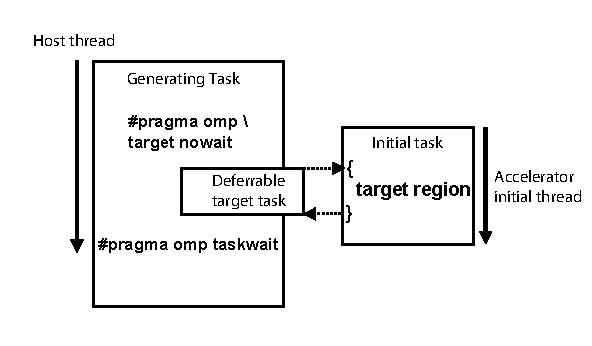
\includegraphics[clip=true,scale=1.00]
         {\ArtDir/device-task-model2.pdf}
     }
\caption{ \textbf{The target task as a deferrable task} -- \small
        The nowait clause makes the target task a deferrable task.  The
        generating task may now be scheduled to execute before the target
        task is complete.  The effect is that the generating task may
        execute in parallel with the target task.
        }
\label{figure:chapter-6-device-task-model2}
\end{figure*}

However, sometimes we want the host device to do useful work in parallel with
the accelerator device. Figure~\ref{figure:chapter-6-device-task-model2} shows
how the \code{nowait} clause solves this problem.  The \code{nowait} clause
changes the default behavior of the target task so that it is no longer an
included task %(see Section~\ref{sec:06.async-exec}).  
With a \code{nowait}
clause, the target task is like any other deferrable task.  

Once a thread suspends execution of a target task, it is available to execute
other tasks, including the original task that generated the target task.  The
effect is that execution of the generating task may continue past the
\code{target} construct and before the associated target region has completed.
The generating task is not stuck waiting for the target task (and thus the
target region) to complete.  The \OMP\ task synchronization features,
introduced in Chapter~\ref{chap:tasking}, may be used to determine
when the target task is complete.

For example, in Figure~\ref{figure:chapter6-nowait} the thread that encounters the
\code{target} construct generates a task and then continues after the
construct to execute the function \code{F()}.  The target task
and the function \code{F()} are potentially executed in parallel.  The host
thread then waits at the \code{taskwait} construct to ensure that the target
task has completed.

\begin{figure*}[!tbh]
\begin{verbatim}
 1 #pragma omp target map(a,b,c,d) nowait // Generate target task
 2 {
 3   #pragma parallel for
 4   for (i=0; i<N; i++) {
 5     a[i] =  b[i] * c + d;
 6   }
 7 } // End of target
 8 
 9 F(b); // Execute in parallel with target task
10
11 #pragma omp taskwait // Wait for target task to finish
\end{verbatim}
\caption{ \textbf {Code fragment with a target nowait region} -- \small
          The encountering thread generates a target task 
          and then continues past the target construct
          to execute the function \emph{F()}.
         }
\label{figure:chapter6-nowait}
\end{figure*}

%In Section~\ref{sec:06.async-exec} we will show more asynchronous execution
%examples using the \code{nowait} clause along with the \code{taskwait}
%construct and \code{depend} clause to demonstrate how to coordinate the
%asynchronous execution of target regions by leveraging the power of \OMP\
%tasks.

%-----------------------------------------------------------------------
%------------------------- New subsection ------------------------------
%-----------------------------------------------------------------------
\subsection{Heterogeneous Memory Model}
\label{ssec:06.heterogeneous-memory-model}

\index{Accelerators!Device constructs}
%Code executing on a device is typically not very useful without some data to
%compute on.  
This section provides an overview of the \OMP\ heterogeneous memory model.
The device constructs, clauses, and runtime functions that control how data is shared
between threads executing on the host and an accelerator device are listed below:

\begin{itemize}
  \item Map and Defaultmap Clauses
  \item Target Data Construct
  \item Target Enter and Exit Data Constructs
  \item Target Update Construct
  \item Declare Target Directive
  \item Use\_device\_ptr and Is\_device\_ptr Clauses
  \item Device Memory Functions
%  \item Runtime Functions
%  \begin{itemize}
%    \item \code{omp_target_alloc}
%    \item \code{omp_target_free}
%    \item \code{omp_target_is_present}
%    \item \code{omp_target_memcpy}
%    \item \code{omp_target_memcpy_rect}
%    \item \code{omp_target_associate_ptr}
%    \item \code{omp_target_disassociate_ptr} 
%  \end{itemize}
\end{itemize}

\index{OpenMP clauses!map}
\index{Accelerators!Map clause}
Of these, by far the most important is the \code{map} clause.  Recall from
Chapter~\ref{chap:recap} that variables are shared or private.  As of \OMPfourzero,
variables can also be \emph{mapped}, which is the concept that \OMP\ uses to
describe how data is shared across devices.  The \code{defaultmap} clause can
change the default rules for determining if certain variables are either
private or mapped.  The general concepts of mapped variables
are discussed later in this section.  
The syntax and mechanics of the \code{map} and \code{defaultmap} clauses
are covered in Section~\ref{sec:06.data-mapping-clauses}.

The host and accelerator may have different representations for the address of
a variable.  The \code{use_device_ptr} and \code{is_device_ptr} clauses are
provided for the instances in which this difference in address representation
must be dealt with explicitly.  These device pointer clauses are covered in
Section~\ref{sec:06.Device-pointer-clauses}.

Variable's with static storage (for example, global variables) may be mapped
for the entire program using the \code{declare target} directive, which is
covered in Section~\ref{sec:06.declare-target-construct}.

The \code{target}~\code{data}, \code{target}~\code{enter}~\code{data},
\code{target}~\code{exit}~\code{data}, and \code{target}~\code{update}
constructs are used to reduce the performance overhead of copying data between
the host and an accelerator.  These data-mapping constructs are
covered in Section~\ref{sec:06.data_mapping_constructs}.

The device memory functions are described in detail in
Section~\ref{ssec:02.new_runtime_functions_3} starting on
page~\pageref{ssec:02.new_runtime_functions_3}.  
The \code{omp_target_is_present} function determines if a variable
is mapped.  Otherwise, the other device memory functions 
manage dynamically allocated device memory.  
Section~\ref{sec:06.device-memory-routines} has examples 
that demonstrate how to use these functions.
%These low-level functions are
%essential for more advanced operations.

%-----------------------------------------------------------------------
%------------------------- New subsection ------------------------------
%-----------------------------------------------------------------------
\subsubsection{Mapped Variables}
\label{ssec:06.mapped-variables}
\index{Mapped variable}

\index{Accelerators!Initial thread}
Threads executing on an accelerator can have private variables.  The initial
thread that begins the execution of a target region gets a private instance of
a variable that appears in a \code{private} or \code{firstprivate} clause on the
\code{target} construct.  For a \code{firstprivate} clause, the private variable
is initialized with the value of the original variable from the host thread
that encountered the construct.  Likewise, any automatic (stack)
variables that are declared in a scope contained within the construct
are private to the initial thread.

%How do the host and accelerator threads share variables?  
\OMP\ threads 
share variables that are stored in a single shared memory.  However, 
heterogeneous architectures do not always have memory that is symmetrically shared between
host and accelerator devices.  A very common example of a 
heterogeneous architecture like this is one where the accelerator is a card 
and communication to the accelerator occurs over a PCIE bus. 

As shown in figure~\ref{figure:chapter-6-device-memory-types}, \OMP\ supports
heterogeneous architectures with both distributed and shared memory by \emph{mapping}
variables from the host to an accelerator.
When the host and accelerator device do not share memory, a mapped variable
is copied from the host's memory into the accelerator's local memory.
Mapping hides whether or not a variable is shared by or copied to a device.
Based on a heterogeneous architecture's memory system, the \OMP\
implementation does what is required, either sharing or copying a variable when it
is mapped.

\begin{figure*}[!tbhp]
\centering
\pdfimageresolution 400
\fbox{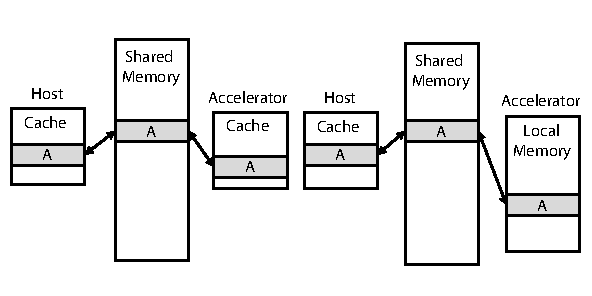
\includegraphics[clip=true,scale=1.00]
         {\ArtDir/device-memory-types.pdf}
     }
\caption{ \textbf{A mapped variable in shared or distributed memory} -- \small
        A mapped variable may be in either shared or distributed memory.
        The OpenMP implementation determines if copies are required.
        }
\label{figure:chapter-6-device-memory-types}
\end{figure*}

\index{Memory consistency!Model} 
How does one ensure that threads on different devices see the same
value of a mapped variable and when?  For the most part, the \OMP\ memory
consistency model as outlined in Chapter~\ref{ssec:01.memory_model}, starting on
page~\pageref{ssec:01.memory_model}, is extended to mapped variables.  

A mapped variable is similar to a shared variable.  Without some 
type of synchronization, two threads executing on
different devices cannot simultaneously access the same mapped variable if
either of the threads writes to the variable.  

\index{OpenMP clauses!map}
\index{Accelerators!Map clause}
Threads executing on different devices may see a consistent value of a mapped
variable at points that are determined by the effects of the \code{map} clause
and the \code{target update} construct.

If memory is distributed, then mapping a variable requires memory allocation,
copy, and flush operations.  The allocation and copy operations are not
required (or are trivial) when memory is shared, but the flush
operation is still necessary.  Although the underlying machinations of variable mapping
is handled by the \OMP\ implementation, it is important to be aware
of the dual-nature of mapped variables to write programs that 
achieve good performance across different architectures.  

%Because the instances of a mapped variable may be in different address spaces,
Because two devices may not share the same address space,
the address of a mapped variable may not be the same on two devices
When a pointer variable is mapped, only the pointer is synchronized, not the
block of memory it points to.  However, array sections may be used to map the
pointed-to memory.

%\index{OpenMP clauses!map}
%\index{Accelerators!Map clause}
%Variables are explicitly mapped using the \code{map} clause (see
%Section~\ref{sec:06.map-clause}).  For variables referenced in a \code{target}
%construct that do not appear in a \code{map}, \code{private},
%\code{firstprivate} or \code{is_device_ptr} clause, data-mapping rules
%determine if they are mapped or private (see
%Section~\ref{ssec:06.defaultmap-clause}).

%Since there might be two copies of the variable, there is a policy for
%maintaining the consistency of the different copies of the variable.
%For example, if a thread on the accelerator writes to a mapped variable, when
%can a thread on the host device see the updated value of the variable?  

%-----------------------------------------------------------------------
%------------------------- New subsection ------------------------------
%-----------------------------------------------------------------------
\subsubsection{Device Data Environments}
\label{ssec:06.device-data-environments}

\index{Accelerators!Device data environment}
\index{Device data environment}
An accelerator has a \emph{device data environment} that contains the set of
all variables currently accessible by threads running on that device.  As we
discussed in the previous section, host threads share variables with target
device threads by mapping them.  Mapping a variable ensures that the variable
is in the data environment of an accelerator.

\index{Device data environment!Orginal variable}
\index{Device data environment!Corresponding variable}
An \emph{original} variable in a host thread's data environment is mapped to a
\emph{corresponding} variable in the accelerator's data environment.
Depending on the availability of shared memory between the host and target
devices, the original and corresponding variables are either the same variable
allocated in shared memory, or they are allocated in different memories and
copy operations are required to keep the original and corresponding variables
consistent. Whether a mapped variable uses shared or distributed memory is 
taken care of by the \OMP\ implementation.

\index{Device data environment!Present in}
There only can be one instance of a variable in a device data environment.  The
\OMP\ implementation keeps track of which variables are mapped.  If a variable
is already \emph{present} in a device data environment, mapping it again will
find the variable is already there and increment a reference count.  It
will not allocate another instance of the variable.

Minimizing the transfer of data between the host and an accelerator is often
critical to getting good performance on heterogeneous architectures.
Repetitively mapping a variable that is reused by multiple \code{target}
constructs is potentially inefficient.  The \code{target}~\code{data},
\code{target enter data} and \code{target}~\code{exit}~\code{data} constructs amortize data
transfers by mapping variables across the execution of multiple \code{target}
constructs.  Further, the \code{declare}~\code{target} construct can map static and
global variables for the whole program.  Once a variable is mapped to an
accelerator, situations can arise where the value of the variable must be
updated from or to the device, and the \code{target}~\code{update}
construct fulfills this need.  The \code{omp_target_is_present} runtime
function is used to test if a variable is mapped.  
\index{Accelerators!omp\_target\_is\_present} 
\index{OpenMP runtime functions!omp\_target\_is\_present} 

%-----------------------------------------------------------------------
%------------------------- New subsection ------------------------------
%-----------------------------------------------------------------------
\subsubsection{Device Pointers}
\label{ssec:06.device-pointers}

\index{Accelerators!Device constructs}
Because shared and distributed memory is supported, the \OMP\ memory model
assumes that the host and accelerator data environments are in different
address spaces.  However, this assumption creates some restrictions on
accessing the address of the variable.
% Ruud - I hope this change is OK
% A programmer using the \OMP\ device constructs must be aware of the different
With the \OMP\ device constructs, the user must be aware of the different
address spaces and be careful when using pointers.  
If the host and accelerator do not share memory, their local memories are in
different address spaces.  When a variable is mapped to an accelerator's data
environment, a copy occurs, and the address of the variable on the accelerator
is not the same as the address of the variable on the host.

Memory addresses are stored in pointer variables.  A host thread cannot access
memory via a pointer variable that contains an accelerator address.  Likewise,
an accelerator thread cannot access memory via a pointer variable that contains
a host address.  
Further, the host and accelerator may have different representations for the
address of a variable.  For example, the value of a memory address might
require 64 bits on a host and 32 bits on an accelerator.

In Figure~\ref{figure:chapter6-devptr1}, the host pointer variable \code{hptr} is
assigned the address of a memory location in the host's address space.  
Mapping \code{hptr} copies the value of the pointer variable to the accelerator. The
access to \code{hptr} at line $6$ in the target region by an accelerator thread is illegal.
The accelerator thread is attempting to access a host address.

Likewise in Figure~\ref{figure:chapter6-devptr2}, the accelerator pointer
variable \code{dptr} is assigned the address of a memory location in the
accelerator's address space.  The access to \code{dptr} at line $7$ by a host thread is illegal.

\begin{figure*}[!tb]
\begin{verbatim}
1   char *hptr = malloc(N);
2
3   // Error - Accessing a host address on accelerator
4   #pragma omp target map(hptr)
5   for (int i=0; i<N; i++)
6     *hptr++ = 0;
\end{verbatim}
\caption{ \textbf {Illegal access of a host memory address } -- \small
          A pointer variable containing a host memory address cannot be
          de-referenced by an accelerator thread.
         }
\label{figure:chapter6-devptr1}
\end{figure*}

\begin{figure*}[!tb]
\begin{verbatim}
1   char *dptr;
2   #pragma omp target map(dptr)
3   dptr = malloc(N);
4
5   // Error - Accessing a device address on host
6   for (int i=0; i<N; i++)
7     *dptr++ = 0;
\end{verbatim}
\caption{ \textbf {Illegal access of an accelerator memory address} -- \small
          A pointer variable containing an accelerator memory address 
          cannot be de-referenced by a host thread.
         }
\label{figure:chapter6-devptr2}
\end{figure*}

\index{Accelerators!Device data environment}
\index{Device data environment}
\index{Accelerators!Device pointer}
\index{Device pointer}
A \emph{device pointer} \index{Accelerators!Device pointer} is a pointer
variable in the host data environment whose value is an object that contains
the address of a storage location in an accelerator's device data environment.  

Note that the value of a device pointer is an object.  How the
value of a device address is represented on a host is not necessarily the same
way that it is represented on an accelerator.  
When a device pointer is referenced in a target construct, the compiler
may need to transform the representation of the device address stored in
the device pointer.

%If a device pointer is stored in
%a host pointer, then the compiler needs to transform the representation of that
%pointer when it is used on the device.  

%The \code{use_device_ptr} and \code{is_device_ptr} 
%clauses are provided for the instances in which the difference in address
%representation between the host and accelerator must be dealt with explicitly.
%\index{Accelerators!Is\_device\_ptr clause}
%\index{OpenMP clauses!is\_device\_ptr}
%\index{Accelerators!Use\_device\_ptr clause}
%\index{OpenMP clauses!use\_device\_ptr}
%We need to indicate that a variable is a device pointer when it is referenced
%in a \code{target} construct.  

%The \code{omp_target_alloc} 
%function, described in detail in Section~\ref{ssec:02.new_runtime_functions_3},
%allocates storage in an accelerator's
%device data environment and returns a device pointer.  The function cannot be
%called inside a target region.  

\index{OpenMP clauses!is\_device\_ptr}
\index{Accelerators!Is\_device\_ptr clause}
In Figure~\ref{figure:chapter6-devptr3}, the \code{omp_target_alloc} function
returns a device address.  The device pointer \code{dptr} must appear in an
\code{is_device_ptr} clause on the \code{target} construct to correctly refer
to it in the target region.  The variable \code{dptr} is private in the target
region.  On entry to the region, the private \code{dptr} variable is initialized
with the accelerator's memory address that corresponds to the original value of
\code{dptr} before the region (the host's representation of the device address).
See Section~\ref{sec:06.Device-pointer-clauses} for more details on device
pointers.

\begin{figure*}[!tb]
\begin{verbatim}
1   int dev = omp_get_default_device();
2   char *dptr = omp_target_alloc(dev, n);
3 
4   #pragma omp target is_device_ptr(dptr)
5   for (int i=0; i<n; i++)
6     *dptr++ = 0;
\end{verbatim}
\caption{ \textbf {Legal access of an accelerator memory address using a device pointer} -- \small
          A device pointer variable that appears in an \texttt{is\_device\_ptr} clause 
          may be de-referenced in a target region.
        }
\label{figure:chapter6-devptr3}
\end{figure*}


%-----------------------------------------------------------------------
%------------------------- New subsection ------------------------------
%-----------------------------------------------------------------------
\subsubsection{Array Sections}
\label{ssec:06.array-sections}
\index{Array section}
\index{Mapped variable!Array section}

Pointer variables are used extensively in C and C++.  The value stored in a
pointer variable is the address of another variable.  As we saw in the last
section, in order to support a variety of systems, the \OMP\ model assumes that
the host and accelerator may not share the same address space. Thus, mapping a
pointer variable by itself is not very useful.  We want to map the pointed-to
variable (the memory that the pointer references). In order to map the
pointed-to variable, we need to know its size.

For C and C++, we need something in the \OMP\ syntax to express the concept of
mapping the pointed-to variables.  This is one of the reasons that \OMPfourzero\
added \emph{array}~\emph{section} syntax for array and pointer 
variables.\footnote{Array sections may also appear in the \code{depend} clause.}

An array section is a subset of the elements in an array.  In \OMP\, array
sections are restricted to a contiguous set of elements.  The C and C++ array
subscript syntax is extended to support an array section expression.  The
array section syntax \code{base[\emph{offset}:\emph{length}]} is described below:

\begin{itemize}

  \item The $base$ is a C or C++ variable name with array, pointer type, or
  in C++, reference to array or reference to pointer type.

  \item The $offset$ is an non-negative integer expression that is an offset
  from the start of the array.  The $offset$ is optional and, if not specified,
  defaults to 0.

  \item The $length$ is a non-negative integer expression that is the length
  of the array section.   If the $base$ variable has a type of array or
  reference to array, then the $length$ is optional and defaults to the
  number of elements in the array.  If the $base$ variable has a type of
  pointer or reference to pointer, then the $length$ must be specified.

%  \item The $stride$ is a (non-negative) integer expression that, when it is
%  greater than one, selects non-contiguous elements from the array.  The
%  $stride$ is optional and defaults to one.  
%  
\end{itemize}

\index{Array section!Pointer-based}
The value of a pointer variable used in an array section is the address of a
pointed-to array variable.  The pointed-to array variable may or may not have
been dynamically allocated.  Even if the pointed-to variable is a single scalar
variable, when it's used in an array section, it is an array of one element.

An array section is \emph{pointer-based} when the $base$ is a pointer variable.
A pointer-based array section is mapped using the following steps: \begin{enumerate}

  \item Create a pointer variable in the accelerator's data environment.

  \item Map the host's pointed-to variable to the accelerator's data
  environment.

  \item Initialize the accelerator's pointer variable with the address of the
  pointed-to variable in the accelerator's address space.

\end{enumerate}

In Figure~\ref{figure:chapter6-array-sections1}, the host pointer variable
\code{hptr} is assigned the address of a storage location in the host's data
environment.  The array section \code{hptr[0:1024]} is then mapped to the
accelerator's data environment.  The 1024 element array pointed to by \code{hptr} is
mapped to the accelerator.  The \code{hptr} pointer variable is not mapped but is
private in the target region and initialized with the address of the pointed-to
array. Compare this to Figure~\ref{figure:chapter6-devptr1}.

\begin{figure*}[!tbhp]
\begin{verbatim}
1   char *hptr;
2
3   hptr = malloc(1024);
4
5   // Map an array section.
6   #pragma omp target map(hptr[0:1024])
7   for (int i=0; i<N; i++)
8     hptr[i] = 0;
9   
\end{verbatim}
\caption{ \textbf {Map a pointer-based array section} -- \small
          Use an array section to map pointed-to memory.
         }
\label{figure:chapter6-array-sections1}
\end{figure*}

\index{Array section!Examples}
\index{OpenMP clauses!map}
\index{Accelerators!Map clause}
Array sections are available in the Fortran base language.  In C/C++, an
array section may appear only as a list item in an \OMP\ \code{map} or
\code{depend} clause.  The C/C++ base language was not extended to support
array sections.  Some examples of array sections in C/C++ are shown
in Figure~\ref{figure:chapter6-map-ptr1}

\begin{figure*}[!tbhp]
\begin{verbatim}
 1 float *p = malloc(N);
 2 float a[N];
 3
 4 // Map pointer based array section
 5 map(p[0:N:1]) 
 6 map(p[0:N])
 7 map(p[:N])
 8
 9 // Map array based array section
10 map(A[0:N:1])
11 map(A[0:N])
12 map(A[:N])
13 map(A[:]) // Size is N
14 
15 // Map array section with offset
16 map(p[32:N-32]
17 map(A[N/2:N/4]
18
\end{verbatim}
\caption{ \textbf {Array section syntax examples} -- \small
          Various usage of array section syntax in C and C++.
         }
\label{figure:chapter6-map-ptr1}
\end{figure*}

\index{Array section!Array slice}
Array sections are also useful for mapping a slice of an array.  It might be
that mapping a very large array exceeds the storage capacity of the
accelerator's local memory.  In this case, we would like to map slices of the
array and then compute on each slice.  Figure~\ref{figure:chapter6-mapslice}
shows how this can be done.

\begin{figure*}[!tb]
\begin{verbatim}
 1 #define BIG 256
 2 #define N (1024*1024)
 3 int a[N*BIG];
 4 
 5 void F(const int c, const int d)
 6 {
 7   for (int k=0; k<N*BIG; k+=N) {
 8     #pragma omp target map(from:a[k:N]) firstprivate(c,d) 
 9     for (int i=0; i<N; i++) {
10       a[k+i] =  k+i * (c + d);
11     } // End of target
12   }
13 }
\end{verbatim}
\caption{ \textbf {Use array section to map a subset of an array} -- \small
          Map a slice of the array \texttt{a} each time through the loop.
         }
\label{figure:chapter6-mapslice}
\end{figure*}

%-----------------------------------------------------------------------
%------------------------- New subsection ------------------------------
%-----------------------------------------------------------------------
\subsection{The Target Construct}
\label{sec:06.target-construct}
\index{OpenMP constructs!Target}
\index{Accelerators!Target}

\index{Accelerators!Initial thread}
The purpose of the \code{target} construct is to offload the execution of code
to an accelerator.  The code in a target region is executed by a new
initial thread.  
The code in Figure~\ref{figure:chapter6-hello} is a simple 
hello world example that uses the \code{target} construct.  

\begin{figure*}[!tbhp]
\begin{verbatim}
 1 #include <stdio.h>
 2 #include <omp.h>
 3 void hello(void)
 4 {
 5   #pragma omp target 
 6   {
 7     if (!omp_is_initial_device())
 8       printf("Hello World from accelerator\n");
 9     else
10       printf("Hello World from host\n");
11   }
12 }
\end{verbatim}
\caption{ \textbf {Example of a target construct } -- \small
          If the initial thread is running on an accelerator, it executes the
          first \texttt{printf()}.
          Otherwise, it is running on the host device and
          executes the second \texttt{printf()}.
          Note that some implementations may not support calling \texttt{printf()} on an accelerator. 
         }
\label{figure:chapter6-hello}
\end{figure*}

\index{Accelerators!omp\_is\_initial\_device}
\index{OpenMP runtime functions!omp\_is\_initial\_device}
The \OMP\ runtime function
\code{omp_is_initial_device} returns true if the code is executing on the
host device.  If there are no accelerators on the system where the code is
running, then the initial thread that executes the target region runs on the host
device.  

\index{Accelerators!Device constructs}
\index{Accelerators!Host fall back} 
Since the initial thread that executes the target region can always 
\emph{fall back} to the host, programs that use device constructs are
portable to systems that do not have accelerators. However, in the following
description of the \code{target} construct it is assumed that the code is
running on a system with at least one accelerator.  

The \code{target} construct syntax in C/C++ and Fortran is given in
Figure~\ref{figure:syntax-target-construct}.  The clauses that are available on
the \code{target} construct are listed in
Figure~\ref{figure:syntax-target-clauses}.

\begin{figure}[!htbp]
\centering
\begin{tabular}{|l|}
\hline
\ompbctarget \ompclauses  \\
\hspace{2em}\emph{structured block} \\
\hline

\ompbftarget \ompclauses \\
\hspace{2em}\emph{structured block} \\
\ompbftargetend \\
\hline

\end{tabular}
\caption{ \textbf{Syntax of the target construct in C/C++ and Fortran} -- \small
          A target region is executed by an
          initial thread running on an accelerator.
          }
\label{figure:syntax-target-construct}
\end{figure}

\index{OpenMP clauses!if}
\index{OpenMP clauses!map}
\index{OpenMP clauses!device}
\index{OpenMP clauses!private}
\index{OpenMP clauses!firstprivate}
\index{OpenMP clauses!is\_device\_ptr}
\index{OpenMP clauses!defaultmap}
\index{OpenMP clauses!nowait}
\index{OpenMP clauses!depend}
\index{Accelerators!If clause}
\index{Accelerators!Map clause}
\index{Accelerators!Device clause}
\index{Accelerators!Private clause}
\index{Accelerators!Firstprivate clause}
\index{Accelerators!Is\_device\_ptr clause}
\index{Accelerators!Defaultmap clause}
\index{Accelerators!Nowait clause}
\index{Accelerators!Depend clause}
\begin{figure}[!htbp]
\centering
\begin{tabular}{|l l|}
\hline
\bciftarget & (C/C++)\\
\bfiftarget & (Fortran)\\
\bmap & \\
\bcdevice & (C/C++)\\
\bfdevice & (Fortran)\\
\bprivate & \\
\bfirstprivate & \\
\bisdeviceptr & \\
\bdefaultmap & \\
\bnowait & \\
\bdepend & \\
\hline

\end{tabular}
\caption{ \textbf{Clauses supported by the target construct} -- \small
          The \texttt{if} and \texttt{device} clauses are discussed in
          Section~\ref{sec:06.which-device}. The \texttt{map} clause is discussed in
          Section~\ref{sec:06.map-clause}.  The \texttt{nowait} and \texttt{depend} clauses are
          discussed in Section~\ref{sec:06.async-exec}.  The \texttt{is\_device\_ptr}
          clause is discussed in Section~\ref{ssec:06.device-pointers} The
          \texttt{defaultmap} clause is discussed in 
          Section~\ref{ssec:06.defaultmap-clause}.
          }
\label{figure:syntax-target-clauses}
\end{figure}

\index{Accelerators!Target task}
The \code{target} construct is a task generating construct.  When a thread
encounters a \code{target} construct a target task is generated on the host
device.  You can think of the target task as a task bound to the host
device that wraps the exection of the target region.  The target task is
complete (on the host) when the target region is complete (on the accelerator).
The \code{nowait} and \code{depend} clauses affect the type and asynchronous
behavior of the target task. 

By default, the execution of the target task is synchronous.  The encountering
thread cannot continue past the target construct until the target task is
complete.  The \code{nowait} clause makes the execution of the target region
asynchronous.  After generating the target task, the encountering thread does
not wait for the target task to complete, but instead it can continue and
execute the code after the \code{target} construct.  Task scheduling via
the \code{taskwait} cosntruct or the \code{depend} clause may be used to
synchronize with the completion of the target task.  The execution model of the
\code{target} construct is covered in detail in
Section~\ref{sec:06.execution-model}.

% Ruud - Changed to a "D" for consistency.
\index{Accelerators!Default-device-var ICV}
\index{ICV!default-device-var}
\index{Accelerators!Host fall back} 
The target region is executed by an initial thread.  Where the initial thread
runs (the host or an accelerator) is determined by the \emph{default-device-var}
ICV. The \code{device} clause can be used to specify a device other than the
default.  The \code{if} clause is available to conditionally fall back to
running the initial thread on the host.

The initial thread gets a private instance of a variable that appears in a
\code{private} or \code{firstprivate} clause on a \code{target} construct.  For
a \code{firstprivate} clause, the private variable is initialized with the value
of the original variable from the host thread that encountered the target
construct.  Likewise, any automatic (stack) variables that are declared in a
scope contained within the target construct are private to the initial thread.

Variables that appear in \code{map} clauses are mapped.  Any assignments 
specified by a \code{map} clause occur when the target task executes. 
If a variable referenced in the \code{target} construct does not appear in a
\code{map}, \code{private}, \code{firstprivate} or \code{is_device_ptr} clause,
then default data-mapping rules determine if and how the variable is mapped
(see Section~\ref{sec:06.data-mapping-clauses}).

\index{Array section!Pointer-based}
C/C++ pointer variables that appear in \code{map} clauses as the base of an
array section are private in the target region. The private variables are 
initialized with the value
of the address of the array section's pointed-to memory in the accelerator's
address space.

The code in Figure~\ref{figure:chapter6-target-mxv} illustrates how to
use the \code{target} construct to offload to an accelerator the matrix times
vector product example taken from \cite{ChapmanEtAl:2007}.  By adding
the \code{target} construct at line $6$, the loop body is offloaded to an
accelerator.

\begin{figure*}[!tb]
\begin{verbatim}
 1 void mxv(int m, int n, double * restrict a,
 2          double * restrict b, double * restrict c)
 3 {
 4 
 5   #pragma omp target map(a[:n],b[:n],c[:n]) firstprivate(m,n)
 6   {
 7     int i, j;
 8     #pragma omp parallel for default(none) \
 9             shared(m,n,a,b,c) private(i,j)
10     for (i=0; i<m; i++)
11     {
12       a[i] = b[i*n]*c[0];
13       for (j=1; j<n; j++)
14         a[i] += b[i*n+j]*c[j];
15     } // End of parallel for
16   } // End of target
17 }
\end{verbatim}
\caption{ \textbf {Example using the target construct to execute the matrix 
                   times vector on an accelerator} -- \small
          The host thread waits for the execution of the target region to
          finish before it continues after the construct.
         }
\label{figure:chapter6-target-mxv}
\end{figure*}

When a host thread encounters the \code{target} construct at line $5$, it generates an
included target task, suspends the current task, and starts executing the
target task.  Because the target task is included, the host thread must
wait for the target region, and thus the target task to complete, before
continuing to execute the statement after the target construct.
Scalar variables that do not appear in a \code{map} clause default to
firstprivate, but for clarity the variables \code{m} and \code{n} are listed 
explicitly in a clause.
Because the variables \code{a}, \code{b}, and \code{c} are pointers, array sections are
required in the \code{map} clause to describe the size of the pointed-to
memory.  The pointer variables themselves are private in the target region.  

The array sections' pointed-to memory is mapped to the accelerator's address
space.
If the host and accelerator do not share memory, storage is allocated in the
accelerator's local memory, and the array sections are copied from the host's
memory to the accelerator's local memory.
The private pointer variables are assigned the address of the array section's
pointed-to memory in the accelerator's address space.
Because the variables \code{i} and \code{j} are declared in a scope enclosed in the
target construct at line $7$, they are private.

The target region is executed by an initial thread running on the default
accelerator.  The initial thread encounters the \code{parallel for}
worksharing construct at lines $8-9$ and becomes the master of a new team of
threads that work together to execute the for-loop at line $10$.  
The variables \code{m}, \code{n}, \code{a}, \code{b}, and \code{c} which were private to the initial
thread are now shared among the threads in the team.  The variables \code{i} and
\code{j} are private to each thread in the team.

If the host and accelerator do not share memory, then when the target region is
complete, the array sections are copied back from the accelerator's local
memory to the host's memory.  The storage allocated in the accelerator's local
memory is then released.  After the target region is complete, the target task
completes and the host thread starts executing again at line $17$ after the
\code{target} construct.

The restrictions on the usage of the \code{target} construct are as follows:

\begin{itemize}

\item A \code{target} construct cannot be nested inside a target region.

\item A \code{target}~\code{data}, \code{target}~\code{update}, \code{target}~\code{enter}~\code{data}, or \code{target}~\code{exit}~\code{data} construct cannnot be nested in a target region.

\item \code{threadprivate} variables cannot be accessed in a target region.

\item In C++ a virtual member function cannot be invoked on an object that was
not constructed on the accelerator.  The object cannot be a mapped variable.

\item In Fortran, if an array section is derived from a variable that has a
\code{POINTER} or \code{ALLOCATABLE} attribute, then the variable cannot be
modified in the target region.

\end{itemize}


